\chapter{Principio de \emph{Hamilton}}

	
\begin{tikzpicture}
	\fill [left color=red!50, right color=teal!50] (0,0) rectangle (6.5,.1);
	\fill [left color=teal!50, right color=blue!50] (6.5,0) rectangle (11.5,.1);
	\end{tikzpicture}

% \var{S}    \fdv{S}{t}

\vspace{10mm}
\begin{adjustwidth}{50pt}{50pt}
\begin{ejemplo}
	Se enuncia brevemente el \emph{principio de Hamilton, de mínima acción o de acción estacionaria}.
	
	Para más información ver apéndice \ref{ApendiceFuncional} Funcional'.



\end{ejemplo}
\end{adjustwidth}

\section{Principio de \emph{Hamilton}}

\begin{myblock}{Principio de Hamilton, de mínima acción o de  acción estacionaria}
Dado el funcional \emph{\textbf{acción}}	 

$$\boldsymbol{
S\ = \ \displaystyle \int_{t_1}^{t_2} \ L(q_j,\ \dot q_j,\ t) \ \dd t
}$$

\vspace{2mm} el sistema (clásico) evolucionará en el tiempo siguiendo las ecuaciones (opuestas a Euler-Lagrange)

$$\displaystyle \pdv{L}{q_j} \ - \ \dv{t} \left( \pdv{L}{\dot q_j} \right) = 0$$

\vspace{2mm} o, lo que es lo mismo,

$$\subrayado{ \ \boxed{\  \boldsymbol{
\displaystyle \fdv{S}{q_j} \ = \ 0 \quad \leftrightarrow \quad \var S = 0 
} \ } \ }$$

\vspace{2mm} la variación de la acción es cero.
\end{myblock}


\subsection{Derivada funcional}
\label{T8Funcional}
\vspace{-5mm}
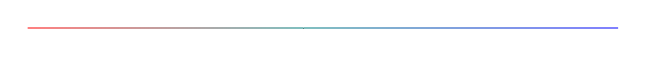
\begin{tikzpicture}
	\fill [left color=red!50, right color=teal!50] (0,0) rectangle (3.5,.01);
	\fill [left color=teal!50, right color=blue!50] (3.5,0) rectangle (7.5,.01);
	\end{tikzpicture}
\vspace{1cm}

\begin{myexampleblock}{ ?`Qué es un funcional?}
Basado en los vídeos comentados en el principio del capítulo.	

	
	
\begin{figure}[H]
		\centering
		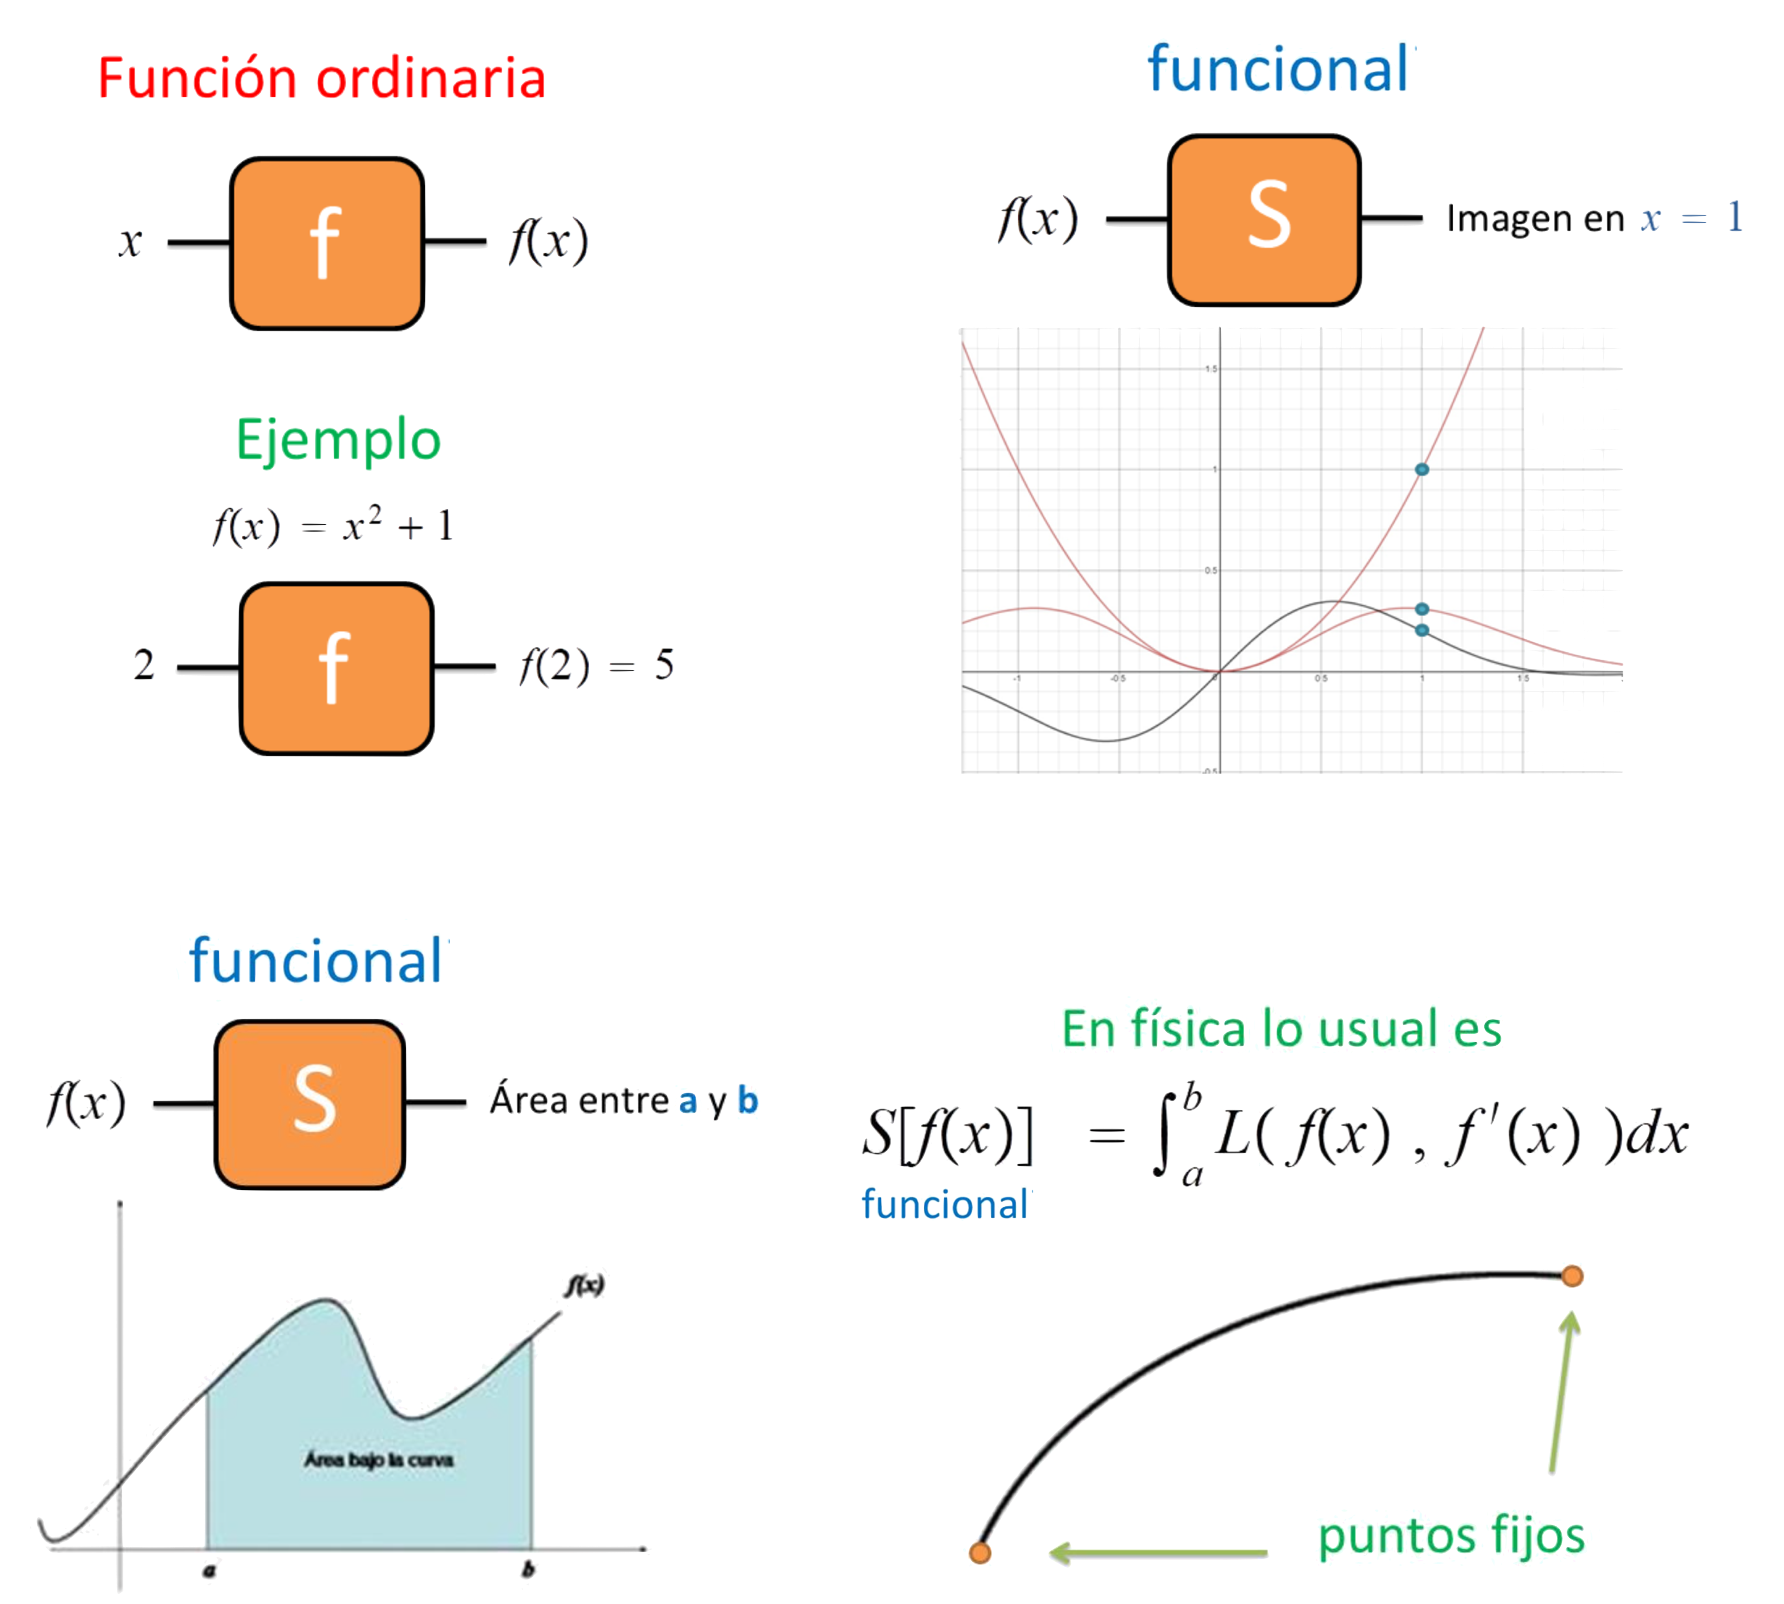
\includegraphics[width=1\textwidth]{imagenes/img08-01.png}
	\end{figure}
	
\begin{center} \rule{200pt}{0.1pt} \end{center}

\begin{figure}[H]
		\centering
		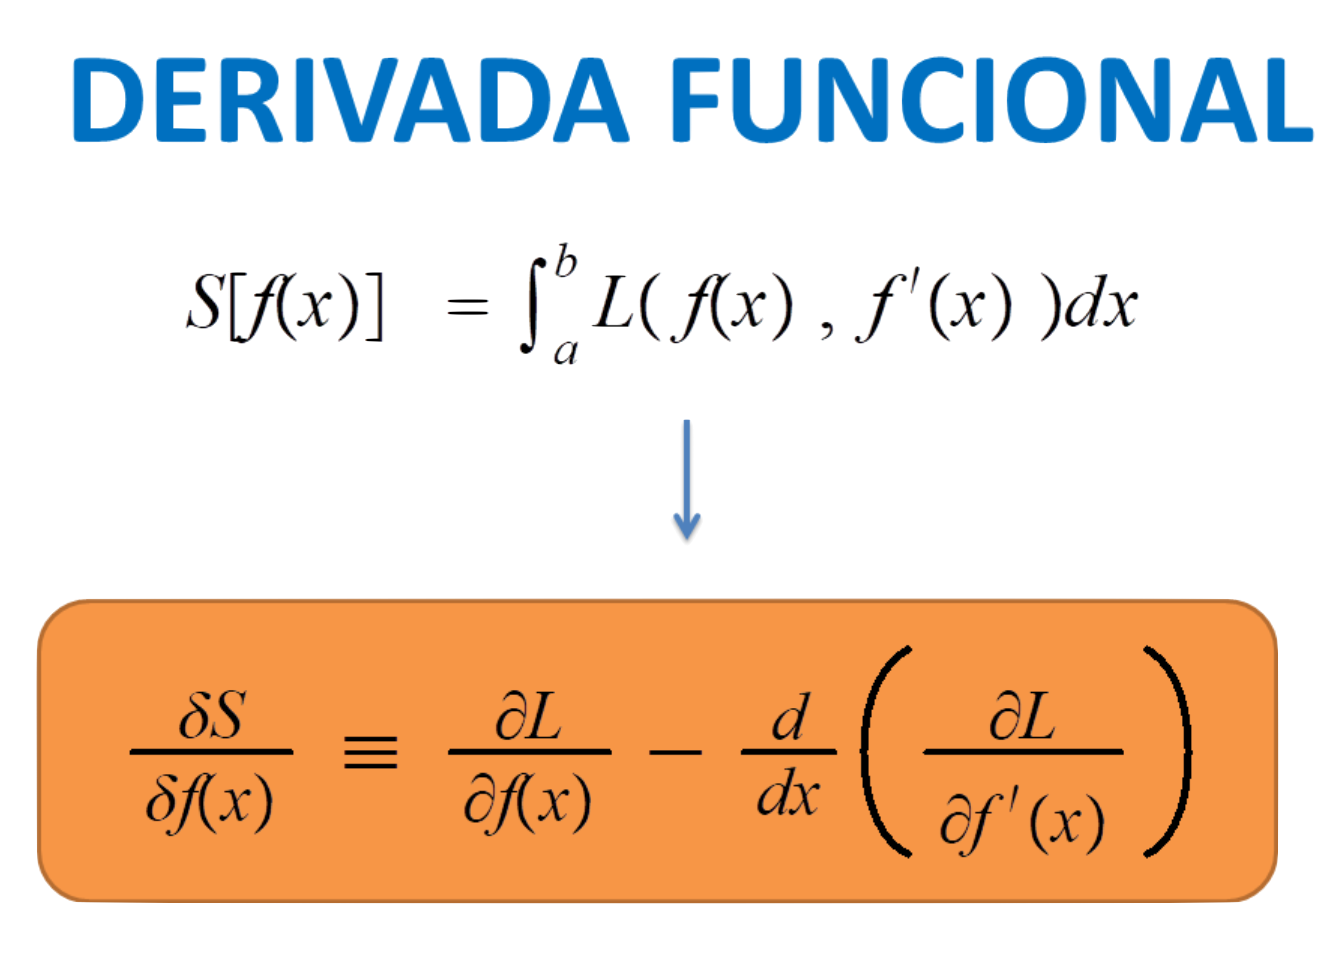
\includegraphics[width=.5\textwidth]{imagenes/img08-02a.png}
	\end{figure}
	
\begin{figure}[H]
		\centering
		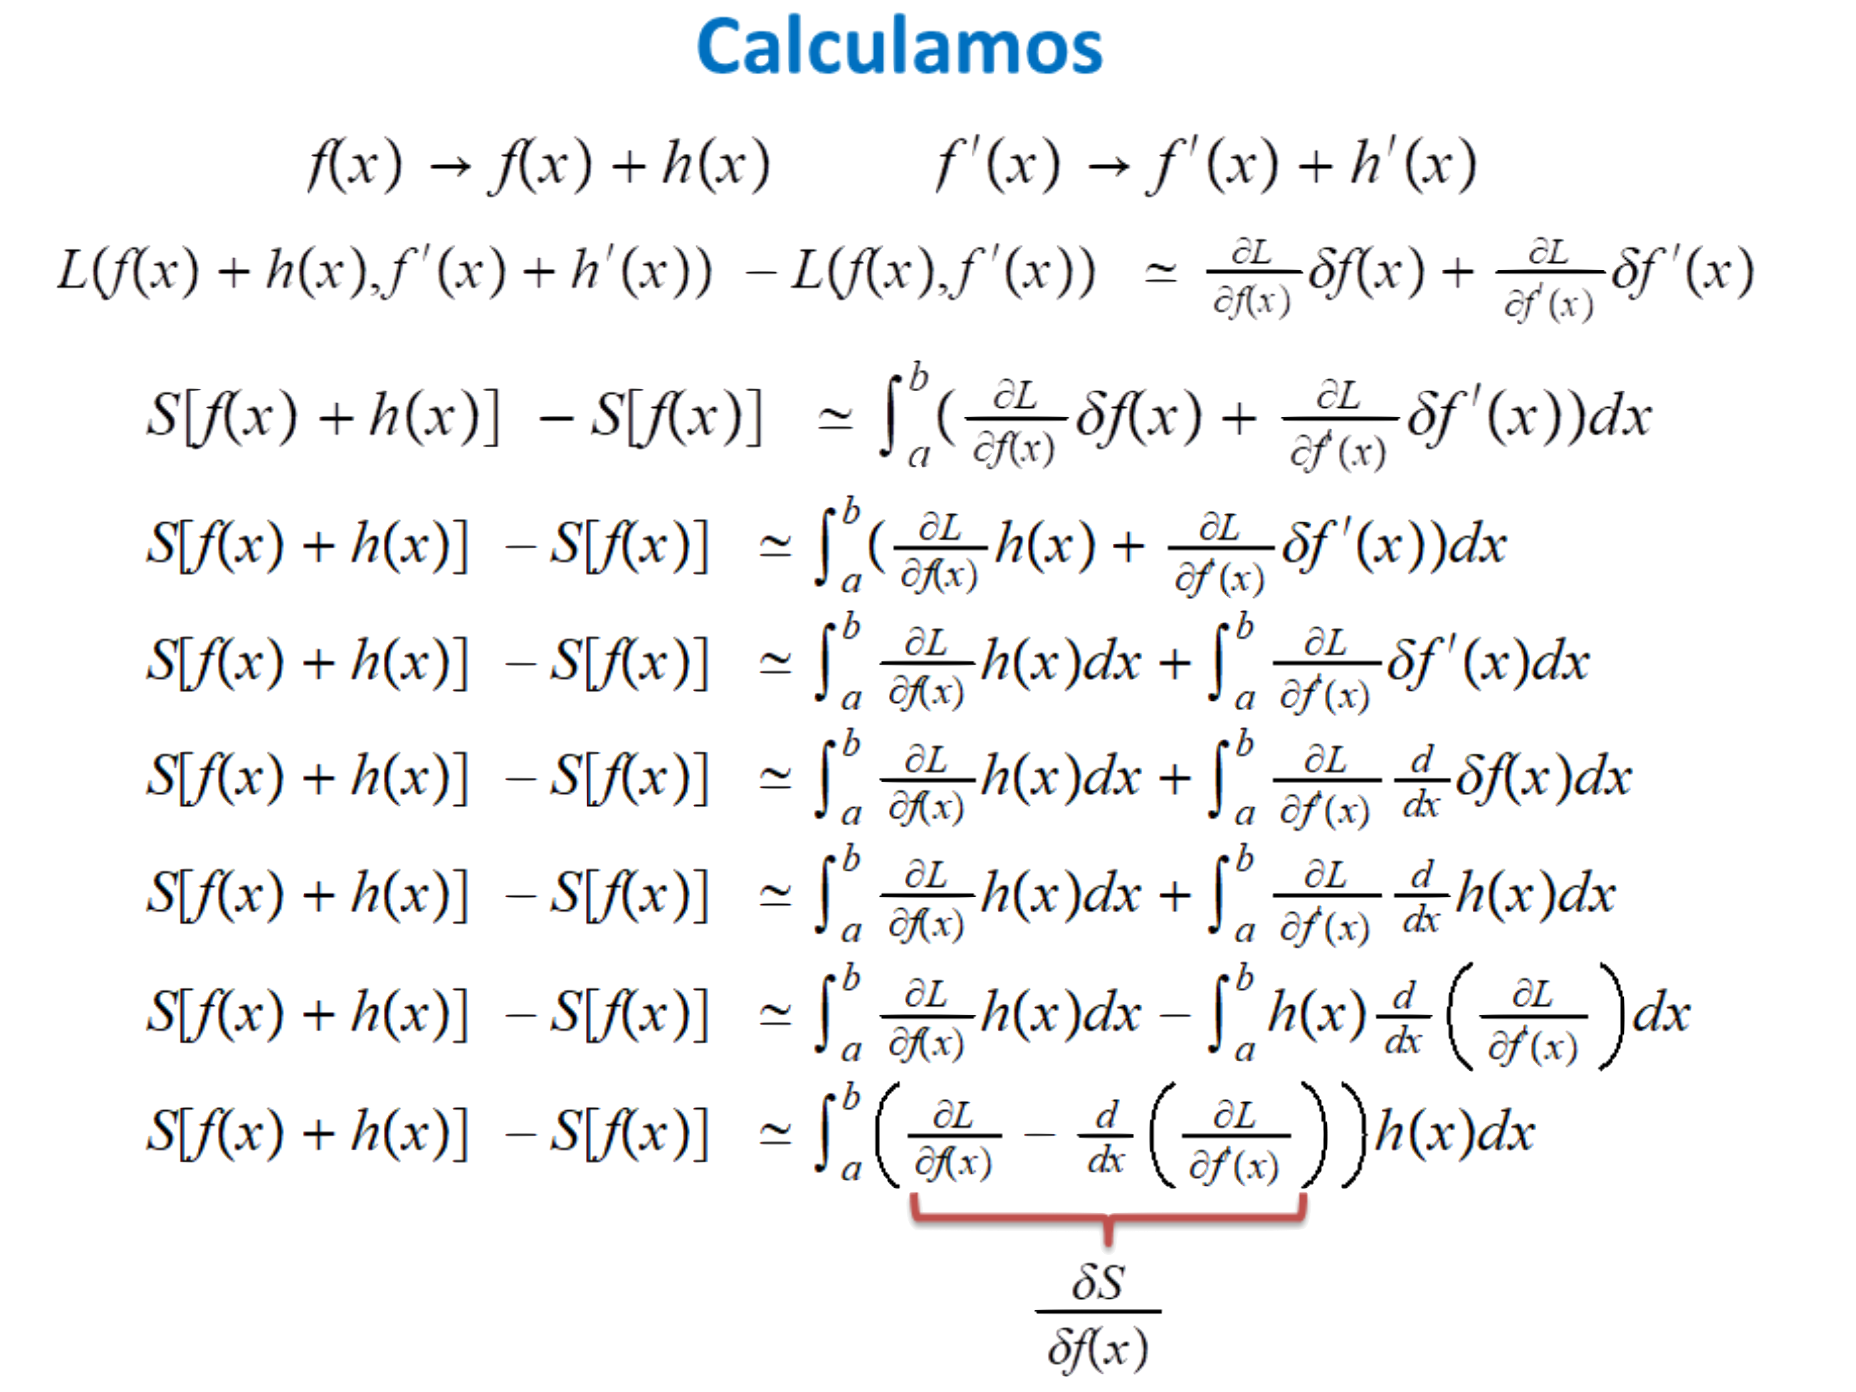
\includegraphics[width=.9\textwidth]{imagenes/img08-02b.png}
	\end{figure}
	
\begin{figure}[H]
		\centering
		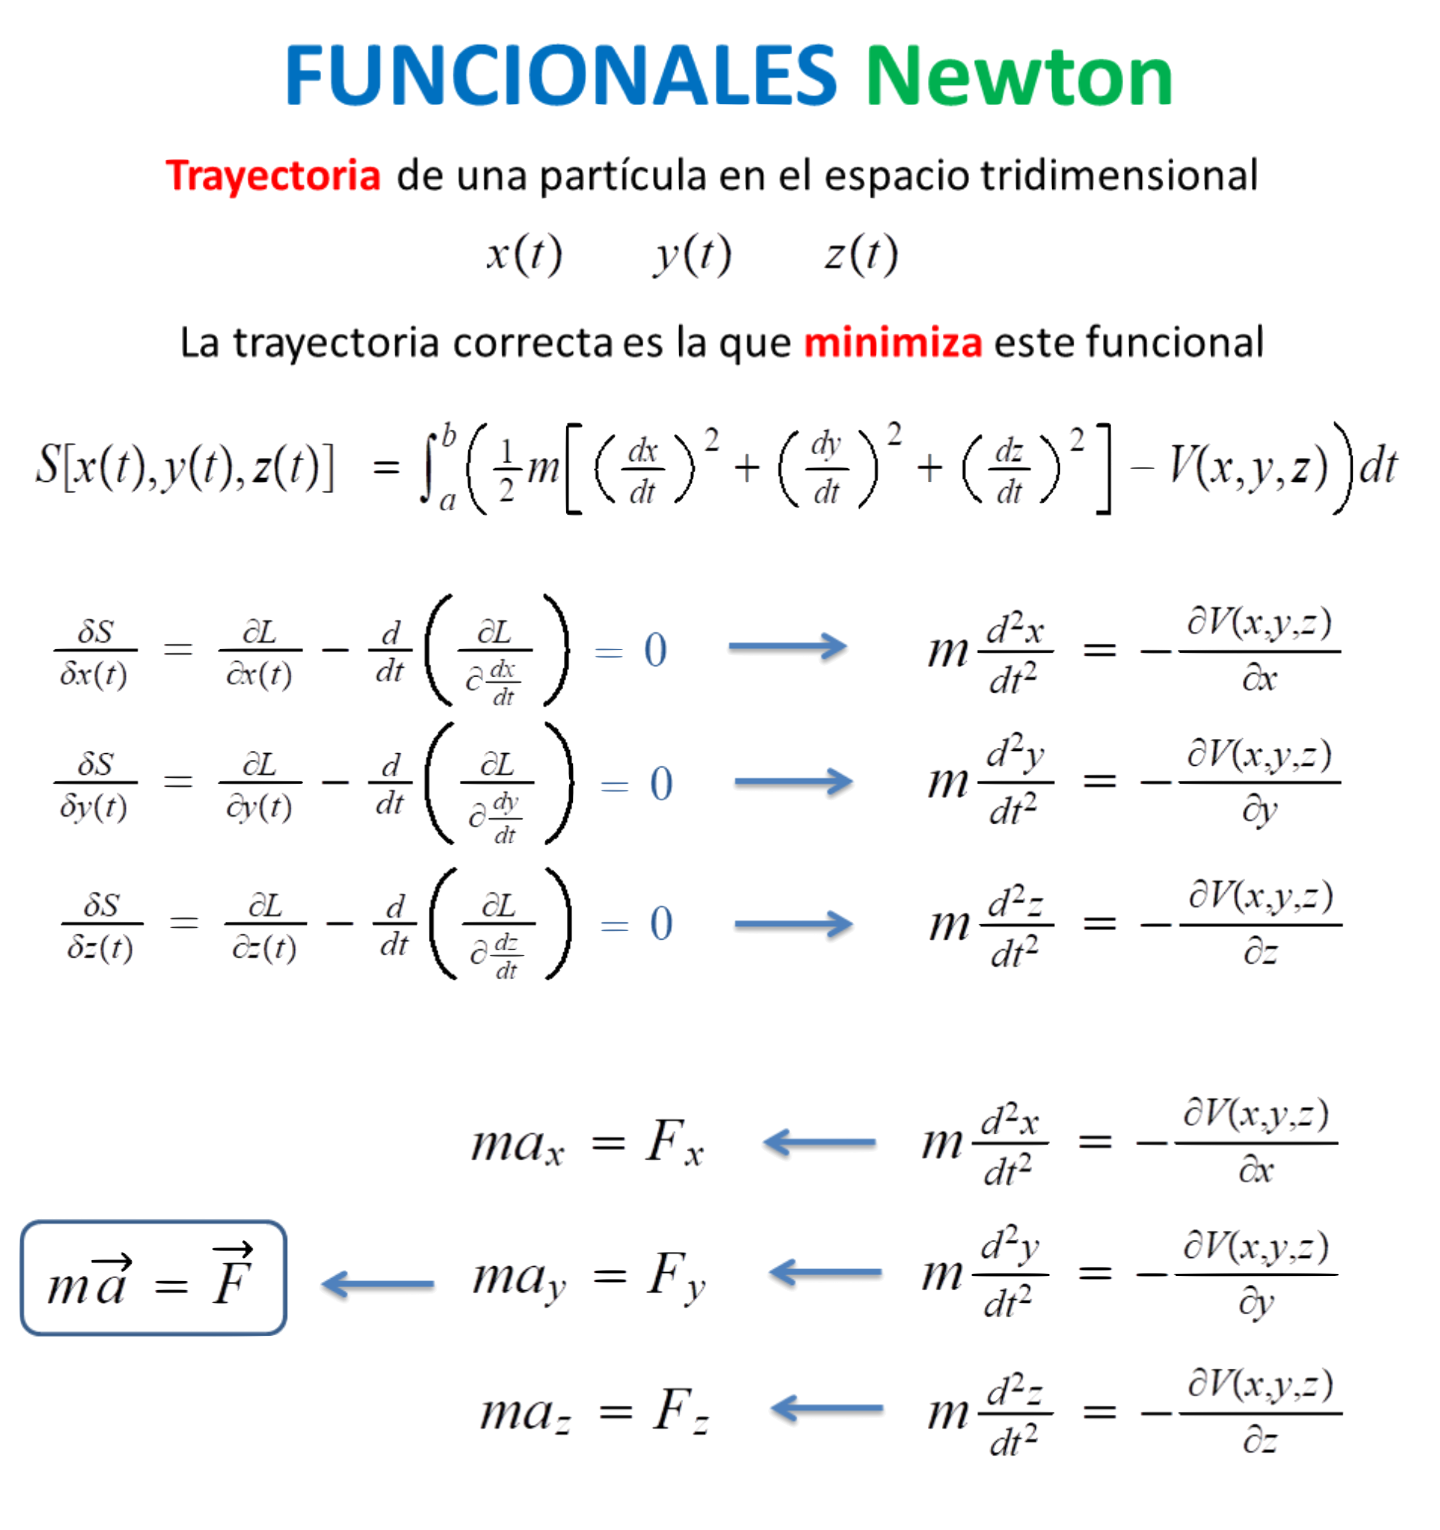
\includegraphics[width=.8\textwidth]{imagenes/img08-03.png}
	\end{figure}

\end{myexampleblock}

\begin{ejemplo}
\vspace{2mm}

Reproduzco, a continuación, el apéndice II de mis apuntes sobre los ``Grupos de Lie'' basados, también, en el video curso de Javier García del mismo nombre. 

\textcolor{teal}{
\begin{footnotesize}
{https://www.youtube.com/playlist?list=PLAnA8FVrBl8DTFTMP8kXbDnRJHQKqfjaw}	
\end{footnotesize} }
\vspace{2mm}
\end{ejemplo}


\newpage
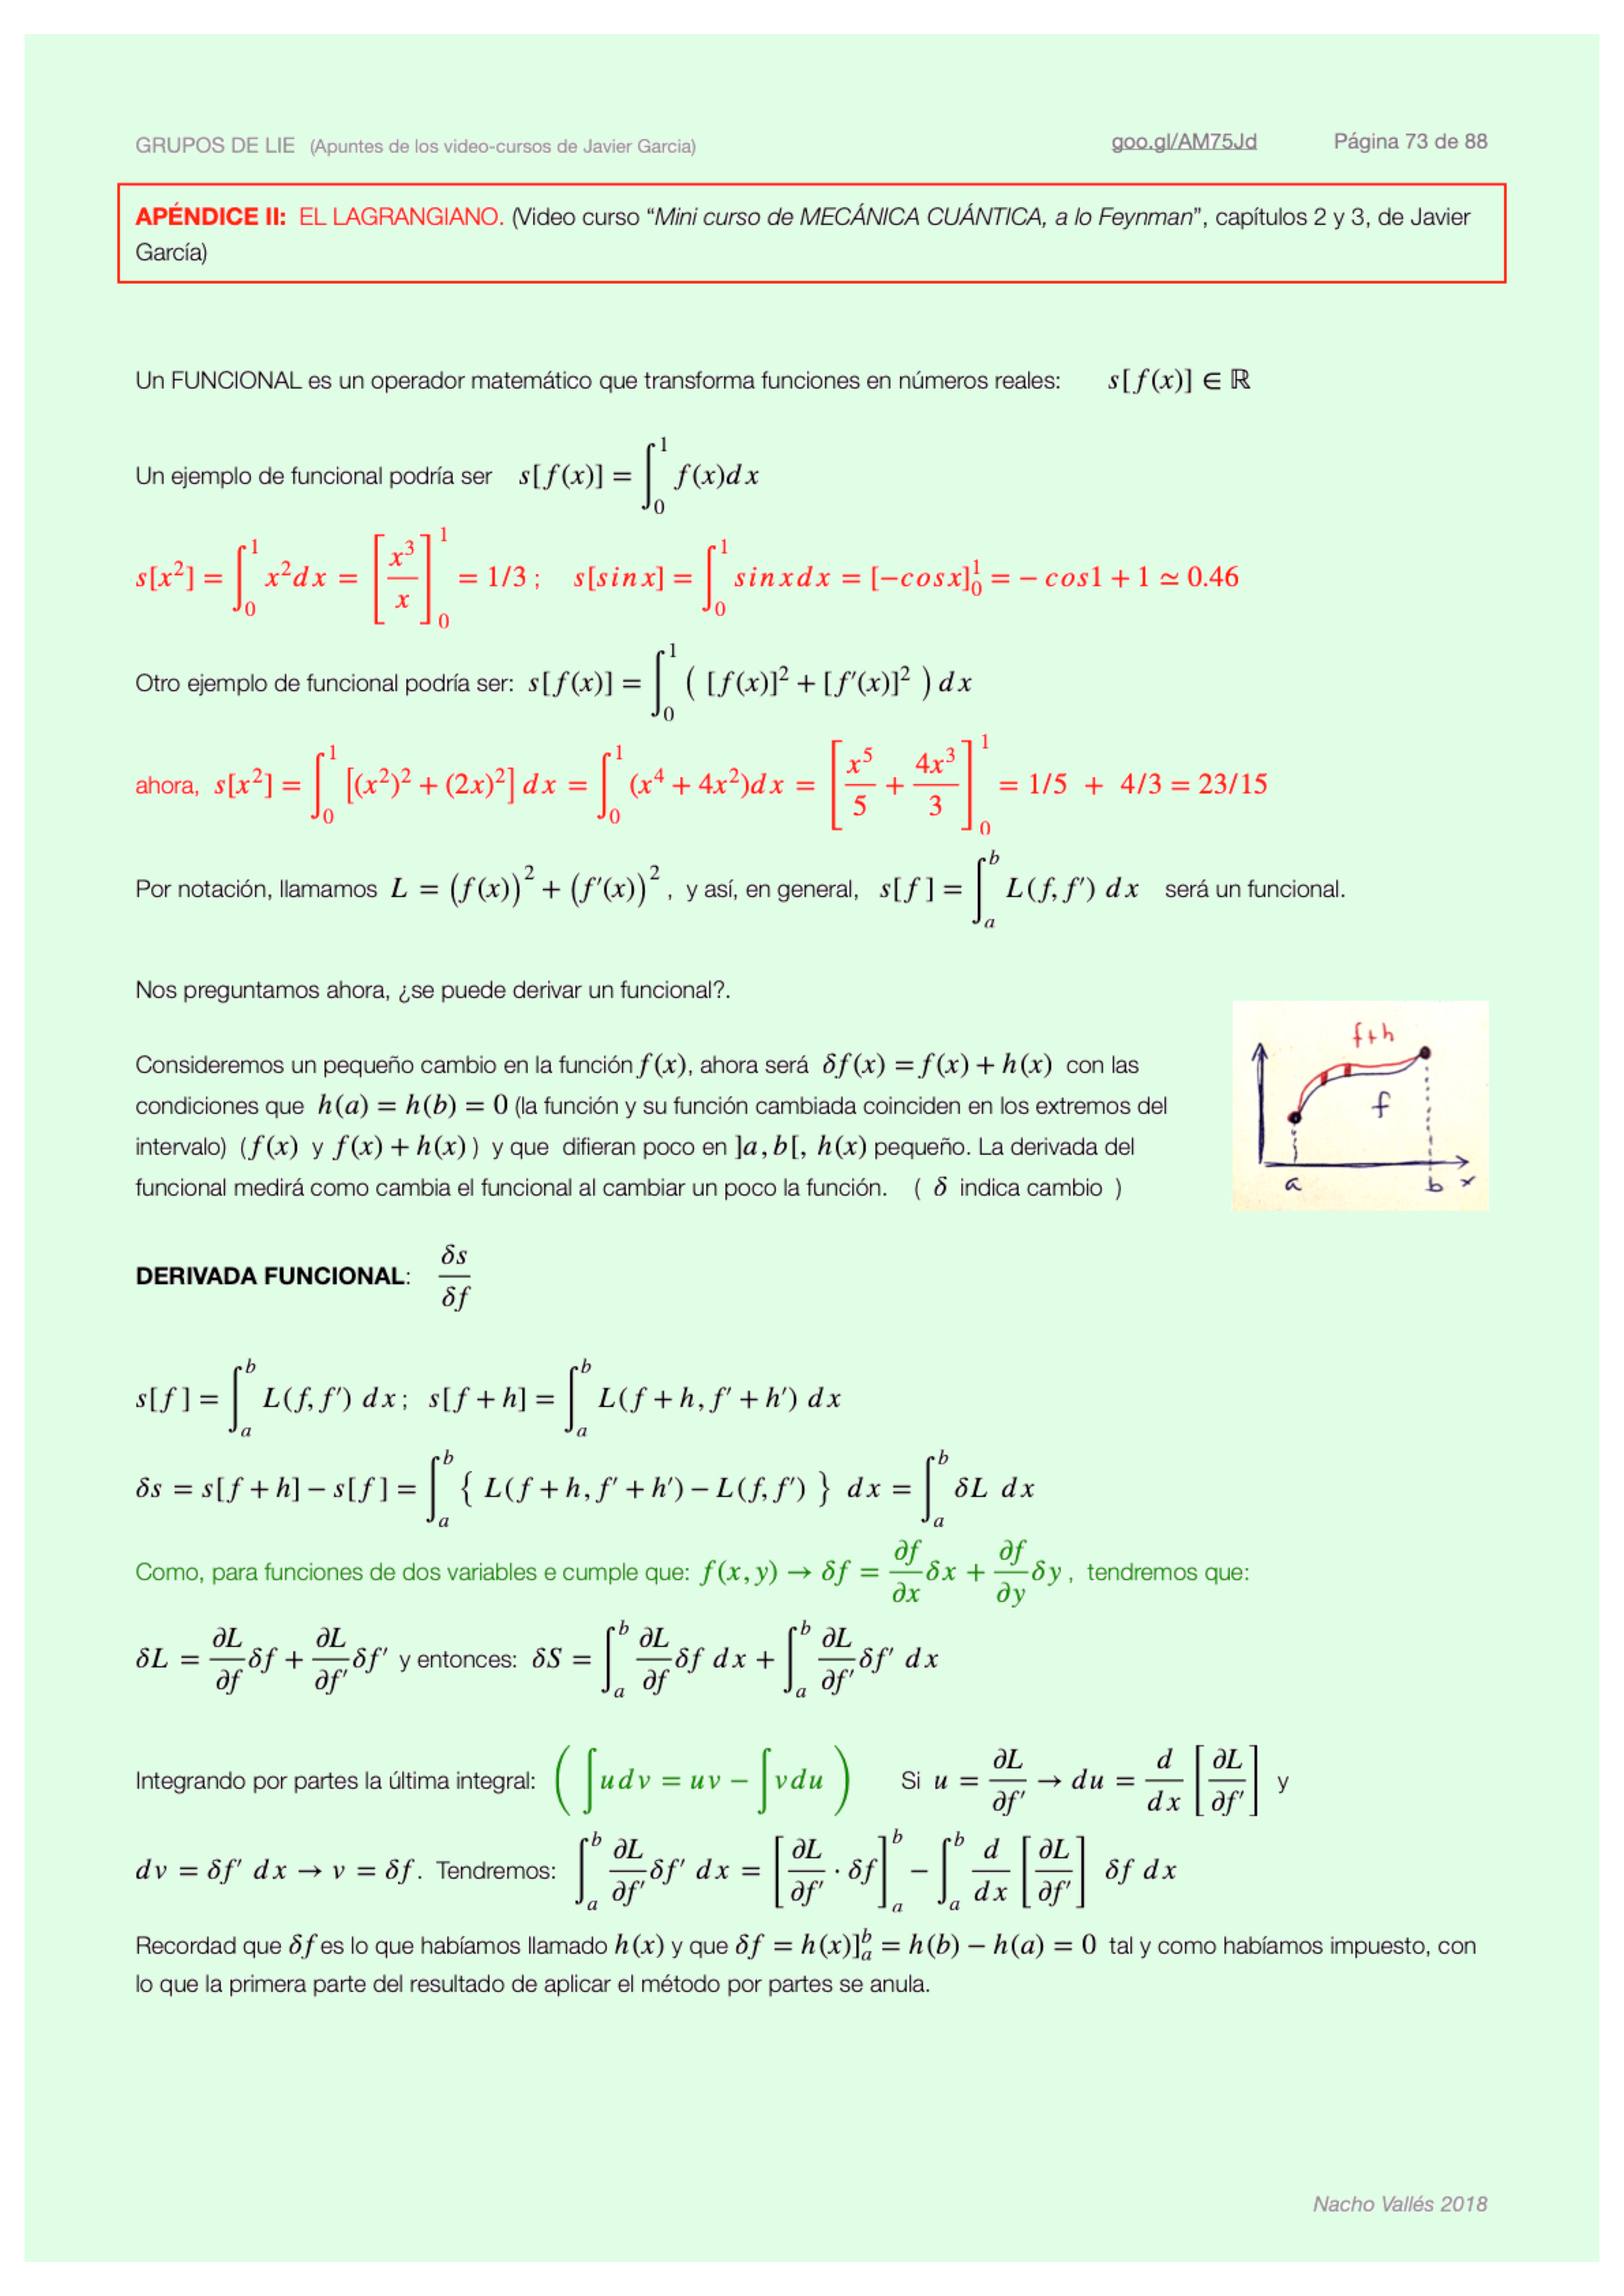
\includepdf[pages=-]{imagenes/derivada-funcional.pdf}





